\documentclass[9pt]{article}

\usepackage{amsmath}
\usepackage{tcolorbox}
% `parskip` removes indentation for all paragraphs: http://tex.stackexchange.com/a/55016
\usepackage{parskip}
% Allows us to color rows / cols of a table.
% See https://texblog.org/2011/04/19/highlight-table-rowscolumns-with-color/
\usepackage{color, colortbl}

\usepackage{graphicx}
\graphicspath{{images/ps2a/}}

\usepackage{hyperref}

\leftmargin=0.25in
\oddsidemargin=0.25in
\textwidth=6.0in
\topmargin=-0.25in
\textheight=9.25in

\definecolor{Gray}{gray}{0.9}

\begin{document}

\begin{center}
  \large\textbf{MIT 18.01 Problem Set 2A Unofficial Solutions}
\end{center}

\begin{tcolorbox}
  \textbf{Q1)} Graph the even and odd functions you found in Problem 1, Part II of PS1. Directly below, graph their derivatives. Do this qualitatively using your estimation of the slope. Do not use the formulas for the derivatives (except to check your work if you want). You can use a graphing calculator to check your answer, provided that you mention it in Problem 0. (Note, however, that you may not use books, notes or calculators during tests, so it is unwise to rely on a graphing calculator here.)
\end{tcolorbox}

\begin{align*}
  \frac{x - 1}{x + 1} &= \frac{x - 1}{x + 1} \cdot \frac{x - 1}{x - 1}\\
                      &= \frac{x^2 - 2x + 1}{x^2 - 1}\\
                      &= \frac{x^2 + 1}{x^2 - 1} - \frac{2x}{x^2 - 1}
\end{align*}

so the even function is $\frac{x^2 + 1}{x^2 - 1}$ and the odd function is -$\frac{2x}{x^2 - 1}$

\begin{center}
  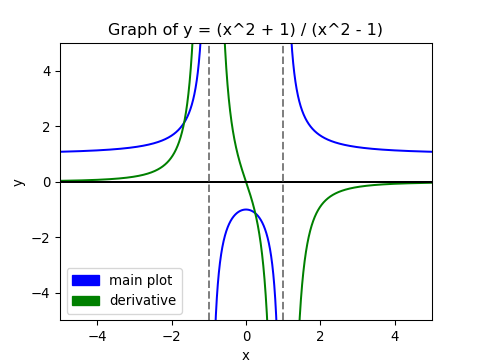
\includegraphics[scale=0.8]{q1_even.png}
\end{center}

\end{document}
